\documentclass[a4paper,twocolumn]{jsarticle}

\usepackage[
    a4paper,
    left=2.0cm,
    right=2.0cm,
    top=2.0cm,
    bottom=2.0cm
]{geometry}
\usepackage{amsmath,amssymb,mathtools,bm}
\usepackage[dvipdfmx]{graphicx}
\usepackage[dvipdfmx]{xcolor}
\usepackage[dvipdfmx,unicode]{hyperref}
\usepackage{pxjahyper}
\usepackage{titlesec}
\usepackage{wrapfig}
\usepackage{multicol}
\usepackage{enumitem}
\usepackage{listings}
\usepackage{float}
\usepackage{caption}
\usepackage{subcaption}
\usepackage{cuted}

\usepackage{tikz}
\usetikzlibrary{positioning}
\usepackage{pgfplots}
\pgfplotsset{compat=1.18}

\usepackage[version=4]{mhchem}
\usepackage{chemfig}

\usepackage{circuitikz}

\usepackage{algorithm}
\usepackage{algpseudocode}

\usepackage{lipsum}

\renewcommand{\theequation}{\arabic{equation}}

\DeclareMathOperator{\sgn}{sgn}
\DeclareMathOperator{\tr}{tr}
\DeclareMathOperator{\diag}{diag}

\hypersetup{
    hidelinks
}

\newcommand{\dif}{\mathrm{d}}
\newcommand{\ee}{\mathrm{e}}
\newcommand{\ii}{\mathrm{i}}

\newcommand{\pd}[2]{\frac{\partial #1}{\partial #2}}
\newcommand{\pdd}[2]{\frac{\partial^2 #1}{\partial #2^2}}
\newcommand{\dd}[2]{\frac{\mathrm{d} #1}{\mathrm{d} #2}}

\newcommand{\vect}[1]{\bm{#1}}
\newcommand{\tensor}[1]{\bm{#1}}

\newcommand{\practiceimage}[2][\linewidth]{%
  \IfFileExists{#2}{%
    \includegraphics[width=#1]{#2}%
  }{%
    \fbox{%
      \parbox[c][28mm][c]{\dimexpr#1-2\fboxsep-2\fboxrule\relax}{%
        \centering\small
        画像ファイル\\未配置%
      }%
    }%
  }%
}

\titleformat{\section}[block]
  {\normalfont\Large\bfseries}
  {\thesection}{1em}{}

\titleformat{\subsection}[block]
  {\normalfont\large\bfseries}
  {\thesubsection}{1em}{}

\titleformat{\subsubsection}[block]
  {\normalfont\normalsize\bfseries}
  {\thesubsubsection}{1em}{}

\titlespacing*{\section}{0pt}{2.0ex plus 0.5ex minus 0.2ex}{0.8ex}
\titlespacing*{\subsection}{0pt}{1.5ex plus 0.4ex minus 0.2ex}{0.5ex}

\lstset{
    language=C,
    basicstyle=\ttfamily\small,
    numbers=left,
    numberstyle=\tiny\color{gray},
    frame=single,
    rulecolor=\color{black},
    backgroundcolor=\color{gray!10},
    breaklines=true,
    showstringspaces=false,
    columns=fullflexible,
    keywordstyle=\color{blue},
    commentstyle=\color{green!50!black},
    stringstyle=\color{red},
    tabsize=4
}

\setlist[itemize]{topsep=4pt,itemsep=2pt,leftmargin=*}
\setlist[enumerate]{topsep=4pt,itemsep=2pt,leftmargin=*}
\captionsetup{font=small}
\setlength{\columnsep}{8mm}
\setlength{\emergencystretch}{1em}
\raggedbottom

\title{%
LaTeXによる基礎演習レポート
}
\author{張毅恒}
\date{\today}

\begin{document}

\maketitle

\begin{abstract}
本稿では，LaTeXを用いて簡単な演習レポートを作成する．
数式，図，表，箇条書き，ソースコード，URL，参考文献を一つの文書にまとめ，
学術的な文書作成で必要となる基本的な表現方法を確認する．
\end{abstract}

\section*{演習1：動作確認}
GitHubから取得した演習ファイルをOverleafでコンパイルし，
PDFを正常に生成できることを確認した．

\section*{演習2：テーマの変更}
タイトルを「LaTeXによる基礎演習レポート」に変更し，
著者名を自分の名前にした．
また，日付には\verb|\today|を設定した．

\section*{演習3：Abstractの挿入}
本レポートでは，タイトルの直後にAbstractを挿入した．
Abstractでは，文書全体で扱う内容を簡潔にまとめ，
読者がレポートの目的を最初に理解できるようにした．

\section*{演習4：数式の挿入}
複素数の指数関数を用いると，三角関数との関係はオイラーの公式
$\ee^{\ii\theta}=\cos\theta+\ii\sin\theta$ として表される．
特に $\theta=\pi$ のとき，次の美しい恒等式が得られる．

\begin{equation}
\ee^{\ii\pi}+1=0
\label{eq:euler_identity}
\end{equation}

また，確率論や統計学でよく現れるガウス積分は次のように表される．

\begin{equation}
\int_{-\infty}^{\infty}\ee^{-x^2}\,\dif x=\sqrt{\pi}
\label{eq:gaussian_integral}
\end{equation}

\section*{演習5：図の挿入}
以下に，自分で用意した画像を挿入した．

\begin{figure}[H]
    \centering
    \practiceimage[4cm]{../figures/kirby_practice.png}
    \caption{演習用に挿入した画像}
    \label{fig:kirby}
\end{figure}

\section*{演習6：表の挿入}
以下に，5行7列の成績表を作成した．

\begin{table}[H]
    \centering
    \resizebox{\linewidth}{!}{%
    \begin{tabular}{|c|c|c|c|c|c|c|}
        \hline
        学籍番号 & 氏名 & 数学 & 英語 & C言語 & AI & 合計 \\
        \hline
        101 & 田中 & 84 & 91 & 78 & 88 & 341 \\
        102 & 鈴木 & 92 & 86 & 81 & 90 & 349 \\
        103 & 伊藤 & 76 & 89 & 85 & 83 & 333 \\
        104 & 中村 & 88 & 82 & 94 & 87 & 351 \\
        \hline
    \end{tabular}
    }
    \caption{成績一覧}
    \label{tab:score}
\end{table}

\section*{演習7：箇条書き}
今回の演習で確認した内容を以下に示す．

\begin{itemize}
    \item 文書の構造を整える
    \item 数式や図表を適切に配置する
    \item 参考文献を引用して一覧に表示する
\end{itemize}

\section*{演習8：ソースコードの挿入}
以下に，平均値を計算するPythonのソースコードを示す．

\begin{lstlisting}[language=Python]
def average(values):
    total = sum(values)
    return total / len(values)

scores = [80, 92, 75, 88]
print(average(scores))
\end{lstlisting}

\section*{演習9：URLの挿入}
以下に，任意のWebページへのURLを挿入した．

\url{https://www.youtube.com/watch?v=dQw4w9WgXcQ}

\section*{演習10：参考文献}
計算機科学の古典的な論文として，Alan Turingによる
``Computing Machinery and Intelligence'' を引用する．
この論文では，機械が知的に振る舞うとは何かという問題が議論されている
\cite{turing1950computing}．
このように，本文中で引用した資料は，文末の参考文献一覧に対応させることで，
どの資料を参照したのかを明確に示すことができる．

引用した文献のBibTeX情報は次の通りである．

\begin{lstlisting}[language={}]
@article{turing1950computing,
  author  = {Alan M. Turing},
  title   = {Computing Machinery and Intelligence},
  journal = {Mind},
  volume  = {59},
  number  = {236},
  pages   = {433--460},
  year    = {1950}
}
\end{lstlisting}

\section*{発展：2段組で大きな図を挿入する}
2段組の文書では，本文を2段組にしながら，図やグラフのみページ全体の幅で
表示することがある．
その場合は，本文の流れの中にページ全体の幅を使う領域を作り，
複数の画像を横並びに配置することができる．
ここでは，配置を確認するためにダミーテキストを多めに入れる．

\lipsum[2-3]

\begin{strip}
    \vspace{-1.0em}
    \centering
    \begin{minipage}{0.44\textwidth}
        \centering
        
\includegraphics[width=\linewidth,height=45mm,keepaspectratio]{../figures/wide_image_kaiju.png}
        \subcaption{画像1}
        \label{fig:wide1}
    \end{minipage}
    \hfill
    \begin{minipage}{0.44\textwidth}
        \centering
        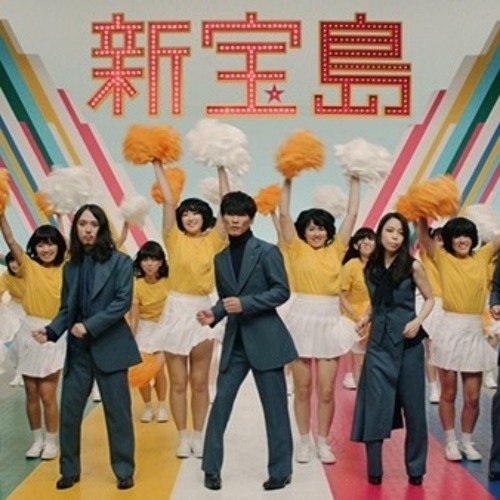
\includegraphics[width=\linewidth,height=45mm,keepaspectratio]{../figures/wide_image_shintakarajima.png}
        \subcaption{画像2}
        \label{fig:wide2}
    \end{minipage}
    \captionof{figure}{画像を横並びにした例}
    \label{fig:wide-images}
    \vspace{-0.5em}
\end{strip}

\lipsum[4-7]

参考文献一覧を以下に示す．

\begin{thebibliography}{1}
\bibitem{turing1950computing}
A. M. Turing,
``Computing Machinery and Intelligence,''
\textit{Mind}, vol. 59, no. 236, pp. 433--460, 1950.
\end{thebibliography}

\end{document}
